\documentclass[12pt]{article}
\usepackage{amsmath,amssymb,relsize,enumitem,fancyhdr,parskip, pgfplots}
\usepackage[margin=1in]{geometry}
\usepackage{CJKutf8}
\newcommand{\Z}{\mathbb{Z}}
\newcommand{\R}{\mathbb{R}}
\newcommand{\N}{\mathbb{N}}
\setlength{\headheight}{28pt}
\pgfplotsset{compat=1.16}
\pagestyle{fancy}
\fancyhf{}
\setlength{\parindent}{0pt}
\fancyhead[c]{Probabilistic and Combinatorial Analysis of Rainbow Board Refresh in \begin{CJK}{UTF8}{min}パズドラ\end{CJK}}
\fancyfoot[c]{\thepage}
        
\begin{document}
\tableofcontents
\section{Introduction}
Consider the standard $5\times 6$ board in the popular mobile game \begin{CJK}{UTF8}{min}パズドラ\end{CJK}. If you apply a rainbow board refresh (assuming all six standard orbs are equally probable), what is the probability of $i$ matches (including skyfalls), for $i\in\N$?
This is a deceptively hard problem as far as I can tell. I hope there is a nice closed form solution, but there probably isn't since it seems to involve partitioning.

Consider the problem with skyfalls disabled.
This limits the number of matches to $i=0,1,\dots,10$.

To consider skyfalls, we may consider the boards as states of a Markov chain (maybe). The expected 

\section{$2\times2$ board with 2-matches}
\subsection{Initial board}
Consider a simplification of the problem:
The board is now $2 \times 2$, and a match occurs when at least two orbs are adjacent to each other.

It is possible to enumerate all of the $6^4=1296$ possible boards.
\begin{itemize}
    \item 0 combos
    \begin{itemize}
        \item Each of the four orbs are distinct colors, so there are $\binom{6}{4}\cdot 4!=360$ boards
        \begin{center}
            \begin{tabular}{|c|c|}
            \hline
            a & b \\
            \hline
            c & d \\
            \hline
            \end{tabular}
        \end{center}
        \item Two of the four orbs are the same color. In order to avoid matches, the two same-colored orbs are diagonal from each other. Therefore there are two possibilities.
        \begin{center}
            \begin{tabular}{|c|c|}
            \hline
            a & b \\
            \hline
            c & a \\
            \hline
            \end{tabular}
            \qquad
            \begin{tabular}{|c|c|}
            \hline
            b & a \\
            \hline
            a & c \\
            \hline
            \end{tabular}
        \end{center}
        This results in $2\cdot\binom{6}{3}\cdot 3!=240$ boards.
        \item Two orbs are the same color and the remaining two orbs are both the same different color. To avoid matches, the same-color pairs must be diagonal from each other, and there is only a single case.
        \begin{center}
            \begin{tabular}{|c|c|}
            \hline
            a & b \\
            \hline
            b & a \\
            \hline
            \end{tabular}
        \end{center}
        This results in $\binom{6}{2}\cdot 2!=30$ boards.
    \end{itemize}
    In total, the probability of 0 combos is $(360+240+30)/1296=35/72$.
    \item 1 combo
    \begin{itemize}
        \item With three colors, we can have the following possibilities:
        \begin{center}
            \begin{tabular}{|c|c|}
            \hline
            a & b \\
            \hline
            a & c \\
            \hline
            \end{tabular}
            \quad
            \begin{tabular}{|c|c|}
            \hline
            a & a \\
            \hline
            b & c \\
            \hline
            \end{tabular}
            \quad
            \begin{tabular}{|c|c|}
            \hline
            b & c \\
            \hline
            a & a \\
            \hline
            \end{tabular}
            \quad
            \begin{tabular}{|c|c|}
            \hline
            b & a \\
            \hline
            c & a \\
            \hline
            \end{tabular}
        \end{center}
        This results in $4\cdot \binom{6}{3}\cdot 3!=480$ boards.
        \item WIth two colors, we have the following possibilities:
        \begin{center}
            \begin{tabular}{|c|c|}
            \hline
            a & a \\
            \hline
            a & b \\
            \hline
            \end{tabular}
            \quad
            \begin{tabular}{|c|c|}
            \hline
            a & a \\
            \hline
            b & a \\
            \hline
            \end{tabular}
            \quad
            \begin{tabular}{|c|c|}
            \hline
            b & a \\
            \hline
            a & a \\
            \hline
            \end{tabular}
            \quad
            \begin{tabular}{|c|c|}
            \hline
            a & b \\
            \hline
            a & a \\
            \hline
            \end{tabular}
        \end{center}
        This results in $4\cdot \binom{6}{2}\cdot 2!=120$ boards.
        \item 
        If all four orbs are the same color, there is only one configuration and $6$ possible boards.
    \end{itemize}
    In total, the probability of 1 combo is $(480+120+6)/1296=101/216$.
    \item 2 combo
    \begin{itemize}
        \item Two adjacent orbs are the same color, and the other two adjacent orbs are another same color.
        \begin{center}
            \begin{tabular}{|c|c|}
            \hline
            a & b \\
            \hline
            a & b \\
            \hline
            \end{tabular}
            \qquad
            \begin{tabular}{|c|c|}
            \hline
            a & a \\
            \hline
            b & b \\
            \hline
            \end{tabular}
        \end{center}
        This results in $2\cdot\binom{6}{2}\cdot 2!=60$ boards.
    \end{itemize}
    The probability of 2 combos is $60/1296=5/108$.
\end{itemize}
\begin{center}
\begin{tikzpicture}
\begin{axis}[
    title=Initial Distribution,
	ylabel=Probability,
	ymax=1,
	enlargelimits=0.15,
	ybar,
	xtick=data,
	xlabel=Combos
]
\addplot coordinates {(0, 35/72) (1, 101/216) (2, 5/108)};
\end{axis}
\end{tikzpicture}
\end{center}
\subsection{Skyfalls enabled}
Now we can consider the board configurations as states of a discrete-time stochastic process. The first thing we should figure out is if this process is Markovian.

The best way to assign states is probably the distinct board configurations as listed above.

\begin{itemize}
    \item Clearly the boards with 0 matches/combos are absorbing states as they do not give rise to any skyfalls, let alone skyfall combos. Any prior board information does not impact the future states since there cannot be any skyfalls.
    \item 
    \begin{itemize}
        \item The three color case leads to three distinct possible remainder boards.
        \begin{center}
            \begin{tabular}{|c|c|}
            \hline
             &  \\
            \hline
            a & b \\
            \hline
            \end{tabular}
            \qquad
            \begin{tabular}{|c|c|}
            \hline
            a & \phantom{a} \\
            \hline
            b & \phantom{a} \\
            \hline
            \end{tabular}
            \qquad
            \begin{tabular}{|c|c|}
            \hline
            \phantom{a} & a \\
            \hline
            \phantom{a} & b \\
            \hline
            \end{tabular}
        \end{center}
        The first board occurs with conditional probability $1/2$, while the other two each occur with probability $1/4$.
        
        What are the possible boards after skyfall? Find out on the next episode...
        \item 
        The two color case...
        \item The single color case is equivalent to a complete board refresh. Therefore all of the boards are once again equally likely.
    \end{itemize}
\end{itemize}

\end{document}